% Propietario conservado: /Users/ruben/Documents/New project/output/REVISION_ARGUMENTAL_APERTURAS_CIERRES_20260915/VIII/spanish_source/ampliacion/centro_frontera.tex
\section{Center, boundary, and vacancies in the nonadic connection}
\label{viii:sec:centro-frontera}
\subsection{The thesis and the order of construction}
The relation between center and boundary acquires mathematical content when one specifies which data are published, which transformations transport them and with what information they are reconstructed. In APP, a residue is accompanied by its quotient; in TRIT, orientation distinguishes operations that an aggregate can merge; in TPK, a turn returns the phase and prolongs memory. The enriched state brings these coordinates together. Its residence in the joint discrete structure of the continuum preserves dependencies between the various subsequent readings.

The path is APP → TRIT → TPK → enriched state → joint discrete structure of the continuum. This development makes local cuts of that path: it does not reconstruct the five consubstantial aspects of the continuum from a spectral form or turn them into five independent modules. The internal constants are received at their publication stage, without using their conventional values to choose seeds, routes or coefficients.

The author's intuition can be expressed thus: \textbf{publication of a value is a projection of a construction; transporting that construction preserves the information that allows its realizations to be distinguished}. The following operations make that statement concrete. The subsequent language of interpolation and orthogonal decomposition proves properties of already specified objects; it does not retrospectively select the APP state.

\subsection{The local crown and reconstruction of the center}
In the positive chart we use

\[
\rho_9(n)=1+[(n-1)]_9,\qquad
q_9(n)=\frac{n-\rho_9(n)}9,
\qquad n=\rho_9(n)+9q_9(n).
\]
The product table is \(P(i,j)=ij\), with \(1\leq i,j\leq9\). Restriction to \(Q=\{3,4,5,6\}^2\) publishes

\[
\left(\rho_9(ij)\right)_{i,j=3}^{6}=
\begin{pmatrix}
9&3&6&9\\
3&7&2&6\\
6&2&7&3\\
9&6&3&9
\end{pmatrix}.
\]

% BEGIN OWNER /Users/ruben/Documents/New project/output/REVISION_ARGUMENTAL_APERTURAS_CIERRES_20260915/VIII/spanish_source/ampliacion/figura_centro_frontera.tex
\begin{figure}[htbp]
\centering
\begin{minipage}[c]{.46\textwidth}
\centering
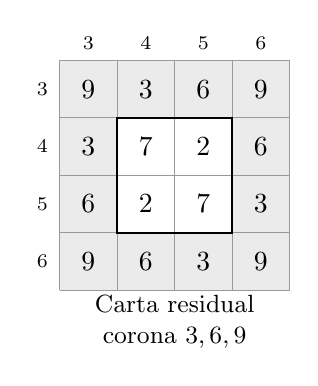
\begin{tikzpicture}[x=.73cm,y=.73cm]
\fill[black!8] (0,0) rectangle (4,4);
\fill[white] (1,1) rectangle (3,3);
\draw[step=1,black!40] (0,0) grid (4,4);
\draw[thick] (1,1) rectangle (3,3);
\foreach \row/\vals in {0/{9,3,6,9},1/{3,7,2,6},2/{6,2,7,3},3/{9,6,3,9}}{
  \foreach \val [count=\col from 0] in \vals{
    \node at (\col+.5,3.5-\row) {\(\val\)};
  }
}
\foreach \v [count=\n from 0] in {3,4,5,6}{
  \node[font=\scriptsize] at (\n+.5,4.3) {\(\v\)};
  \node[font=\scriptsize] at (-.3,3.5-\n) {\(\v\)};
}
\node[font=\small,align=center] at (2,-.55) {Carta residual\\corona \(3,6,9\)};
\end{tikzpicture}
\end{minipage}\hfill
\begin{minipage}[c]{.50\textwidth}
\centering
\begin{tikzpicture}[x=.73cm,y=.73cm]
\fill[black!3] (0,0) rectangle (4,4);
\draw[black!40] (0,0) rectangle (4,4);
\draw[thick] (1,1) rectangle (3,3);
\foreach \x/\y/\v in {.5/3.5/9,3.5/3.5/18,.5/.5/18,3.5/.5/36,
  1.5/2.5/16,2.5/2.5/20,1.5/1.5/20,2.5/1.5/25}{
  \node at (\x,\y) {\(\v\)};
}
\draw[-{Stealth},black!60] (.85,3.15) -- (1.22,2.78);
\draw[-{Stealth},black!60] (3.15,3.15) -- (2.78,2.78);
\draw[-{Stealth},black!60] (.85,.85) -- (1.22,1.22);
\draw[-{Stealth},black!60] (3.15,.85) -- (2.78,1.22);
\node[font=\small,align=center] at (2,-.55) {Lifted boundary\\and multiaffine interpolation};
\end{tikzpicture}
\end{minipage}
\caption{The same chart in two readings. On the left, the radical crown surrounds the block \(B_c\). On the right, the four integer corners determine the interior values under the multiaffine law. Their corner residues coincide, but the quotients \((0,1,1,3)\) distinguish the lift.}
\label{viii:fig:centro-frontera}
\end{figure}

% END OWNER


\Needspace{6\baselineskip}
Its inner block is

\[
B_c=\begin{pmatrix}7&2\\2&7\end{pmatrix}.
\]
The perimeter of this chart contains twelve positions: four with value \(3\), four with \(6\) and four with \(9\); their sum is \(72\). A radical crown becomes visible around the central block. The global electronic center is \((5,5)\), the unique fixed point of inversion of the complete APP; its position is not changed by choosing this local chart, whose geometric center is at \((4.5,4.5)\).

\begin{proposition}[Recovery from the lifted boundary]
\label{viii:prop:centro-frontera-recuperacion}
Let \(F(x,y)=a+bx+cy+dxy\) be a multiaffine law in the chart \([3,6]^2\). For \(t=(x-3)/3\) and \(u=(y-3)/3\),

\[
\begin{aligned}
F(x,y)={}&(1-t)(1-u)F(3,3)+(1-t)uF(3,6)\\
&+t(1-u)F(6,3)+tuF(6,6).
\end{aligned}
\]
\end{proposition}
\begin{proof}
For fixed \(y\), affinity in \(x\) recovers \(F(x,y)\) from \(F(3,y)\) and \(F(6,y)\). Affinity in \(y\) recovers each of those two values from its endpoints. Composition gives the formula. In particular, the four corners determine the entire chart within the declared space of laws.
\end{proof}

For the product, the four lifted values are \(9,18,18,36\). Their positive residues are all \(9\), but their quotients are \(0,1,1,3\). The formula recovers \(16,20,20,25\) at the interior positions; its residual publication gives \(7,2,2,7\). In this way, the boundary determines the interior \textbf{while preserving the law and the lift}. Interpolation is performed before modular reduction: one does not divide by \(3\) in \(\mathbb Z/9\mathbb Z\), where \(3\) is not invertible.

This specifies the meaning of “preserving the information of the center.” The residual crown alone does not individualize all lifts: \(F\) and \(F+9\) have the same residues along the entire boundary and different lifted values. The residue–quotient pair removes that ambiguity within the indicated reconstruction. The assertion is proved for multiaffine laws; extending it to complete states also requires preserving the operators, routes, and memory acting on them.

Multiaffine recovery is a \textbf{new formalization of the preexisting authorial architecture}. The charts and their readings are results recovered from the corpus; this explicit presentation of their inverse is not attributed as an independent historical discovery.

\subsection{Sum, product, and the three values of discrete curvature}
The multiplicative rows are constructed by additive accumulation. The difference between the two sheets appears when both coordinates are varied simultaneously. With unit differences,

\[
\Delta_x\Delta_y(x+y)=0,
\qquad
\Delta_x\Delta_y(xy)=1.
\]
The same property is recovered on the lifted boundary:

\[
\frac{P(6,6)-P(6,3)-P(3,6)+P(3,3)}{3\cdot3}=1;
\]
for \(S(x,y)=x+y\), this quotient equals \(0\). The product records the cross variation that the sum does not introduce. The corpus expresses the oriented version through

\[
\mathcal F(T_x,T_y)=\Delta_x\Delta_yT_y-\Delta_y\Delta_xT_x,
\]
\[
\mathcal F(S,S)=\mathcal F(P,P)=0,
\qquad \mathcal F(S,P)=+1,
\qquad \mathcal F(P,S)=-1.
\]
The order of the sheets distinguishes the sign. The formulation “the sum accumulates and the product folds or unfolds” rests here on a verifiable operation: modular projection preserves a residue; lifting recovers the quotient recording what was exceeded. Discrete curvature additionally records the order of the variations. This finite difference is not identified with a differential curvature of a physical space without its corresponding realization map.

\subsubsection*{The global radical cross}
In \(R=\mathbb Z/9\mathbb Z\), the ideal \(\mathfrak m=\{0,3,6\}\) satisfies \(\mathfrak m^2=0\). Its positive publication is \(\{9,3,6\}\). The cross

\[
(\mathfrak m\times R)\cup(R\times\mathfrak m)
\]
has \(27+27-9=45\) positions. The intersection contains nine values \(9\), summing to \(81\); the remaining arms have twelve values of each class \(3,6,9\), summing to \(216\). The total is

\[
297=216+81=3(72+27)=3\cdot99.
\]
Four boundaries are distinguished: the local perimeter of twelve positions, the radical cross of forty-five, the gnomon of seventeen completing \(8^2\) to \(9^2\), and the cubic crown of \(271\). Each has its own domain and operation. The tritic quotient \(R/\mathfrak m\) preserves a class; transporting the state requires accompanying it with the lifted data and their history.

\subsection{The 72–27 and 77–22 readouts and the 729–271 completion}
The ordered rows of \(B_c\) are published decimally as \(72\) and \(27\); its diagonals as \(77\) and \(22\). This yields

\[
72+27=77+22=99.
\]
In the cubic completion, counting the interior, faces, edges, and vertex gives

\[
1000=729+243+27+1=729+271,
\]
\[
999=729+243+27=729+270.
\]
The coincidence of readouts is expressed while preserving the decimal remainder:

\[
729=10\cdot72+9,\qquad271=10\cdot27+1.
\]
Therefore, the two-dimensional reading publishes \((72,27)\); the cubic reading publishes \(((72,9),(27,1))\). The pair of remainders \((9,1)\) distinguishes the prolongations that would share the same quotient. The chart constructions are carried out first; those publications are then compared. The identity of the integers does not reverse that causal order.

The chapter on integer channels provides another specific composition. With the internal counts \(\Delta=54\), \(\nu=\Delta/2=27\), and \(\Theta=5\nu=135\), it obtains

\[
\mathcal C_\alpha=\nu^2=729,
\qquad \mathcal C_e=2\Theta+1=271.
\]
Here \(\nu\) is the new name for the local integer denoted by \(\kappa\) in that source, to distinguish it from the rational readout of the dodecaphase record. The channels are integer objects; their identification with the constants passes through the regional readouts and the corresponding closure, not through the first digits of an expansion. This comparison uses the integer channels and does not require the subsequent angular realization.

For the oral reference to a fraction of \(\pi\), the located source contains

\[
\frac{396}{126}=\frac{22}{7},\qquad
396=18+72+108+198,\quad126=18+108.
\]
It is a rational ratio of alternating rings. This ring ratio is an exact rational reading; its role is distinguished from the regional publication of \(\pi\).

\subsection{The electronic center and its conjugate vacancies}
The inversion of the positive APP is \(\rho(r,c)=(10-r,10-c)\). Its unique fixed point is \((5,5)\). In the central additive fiber,

\[
\mathcal F_{10}=\{(5+t,5-t):t\in\mathbb Z,\ |t|\leq4\},
\]
the product equals \(25-t^2\). Preserving its central residue requires \(t^2\equiv0\pmod9\), equivalent to \(3\mid t\). The only positions are therefore

\[
(5,5),\qquad(8,2),\qquad(2,8).
\]
If \(\mathcal A\) preserves the residue–quotient pair on each sheet,

\[
\begin{aligned}
\mathcal A(5,5)&=((1,1),(7,2)),\\
\mathcal A(8,2)=\mathcal A(2,8)&=((1,1),(7,1)).
\end{aligned}
\]
The two vacancies preserve the additive readout and the multiplicative residue; the product quotient decreases by exactly one unit. The mirror \(t\mapsto-t\) exchanges their positions. The residual value does not distinguish their routes, whereas orientation does preserve them. This is a precise realization of the connection indicated in the note: \textbf{a vacancy is individualized by a relation to the center and by a recorded defect, not by being a cell without information}.

The initial electronic orientation \((h_0,v_0)=(1,1)\), reversed every \(27\) steps, subsequently publishes the dodecaphase signature \((+++\,---\,+++\,---)\). This is an orientation record, distinct both from the position \((5,5)\) and from the following product signature.

\subsubsection*{The signature 555555 and the memory enabling its prolongation}
For \(U_j=100d_{1j}+10d_{2j}+d_{3j}\), the readout

\[
\mathcal E_\times(U)=([d_{2j}-d_{1j}]_{10})_{j=1}^{6}
\]
applied to the transverse region

\[
U_\pi^\perp=(501,614,498,169,272,272)
\]
produces \(555555\); its reduction \(\Psi(U)=(-U_j\bmod3)_j\) produces \(010211\). The signature has twenty-four product representatives. Transport separates them into three sheets of eight: after advancement, \(555177\), \(555717\), and \(555771\) appear. The congruence stable under advancement and half-turn refines the twenty-six signatures into twenty-eight classes, with histogram \(27\cdot8+108=324\). This expresses why sheet memory must be retained to continue a signature that initially coincides.


% BEGIN OWNER /Users/ruben/Documents/New project/output/REVISION_ARGUMENTAL_APERTURAS_CIERRES_20260915/VIII/spanish_source/ampliacion/memoria_firma_555.tex
\begin{definition}[Signature readout and transport of representatives]
\label{viii:def:firma555}
Let \(\mathcal X_\times=D_9^2\times\{N,E,S,O\}\), of cardinality \(324\).
Advancement \(P\) moves one cell in the stored direction, and the half-turn
\(H\) reverses that direction. The readout uses
\[
\ell_9(1,2,4,8,7,5)=(0,1,2,3,4,5),\qquad
\ell_9(3)=\ell_9(6)=\ell_9(9)=0.
\]
In each of six windows of nine steps,
\(\ell_9(\rho_9(ij))\) is evaluated before the product advancement selected by TRIT at
times \(2,5,8\pmod9\). The sum in each window is reduced modulo
\(10\). After steps \(27\) and \(54\), the direction is reversed.
The rule determines \(E_{\rm sig}(x)\) from the position and direction
of \(x\), with the kernel's time conventions.
\end{definition}

\begin{proposition}[Minimal stable refinement of the signature]
\label{viii:prop:firma555}
Starting from equivalence by signature \(\sim_0\), the iteration
\[
x\sim_{n+1}y\ \Longleftrightarrow\
x\sim_n y,\quad Px\sim_n Py,\quad Hx\sim_n Hy
\]
terminates and produces the coarsest stable congruence refining the signature.
On the preceding domain the census is \(26\to28\to28\); the fiber of
\(555555\) separates into three classes of eight representatives.
\end{proposition}
\begin{proof}
At each step, a partition of a finite set is refined. The process
stabilizes after finitely many splittings. At the fixed point,
equivalence is preserved under \(P\) and \(H\). If a stable congruence
refines \(\sim_0\), it refines each \(\sim_n\) by induction: its images
under both operators remain equivalent. It therefore refines the fixed
point obtained, proving its minimality in added information.

The finite enumeration applies the definition to the \(81\) positions and the
four orientations. Their six sums modulo \(10\) are grouped first, and
then the triple consisting of the class of \(x\), that of \(Px\), and that of
\(Hx\), until stabilization. The resulting histogram is
\(27\cdot8+108=324\), and the only signature splitting is the one indicated.
The following representatives make the three images explicit:
\[
\begin{array}{c|c|c}
x&E_{\rm sig}(x)&E_{\rm sig}(Px)\\\hline
(3,5,N)&555555&555177\\
(3,4,N)&555555&555717\\
(3,4,S)&555555&555771
\end{array}
\]
The complete rule and its executable enumeration are preserved in the
reproduction package; the witnesses in the table also show that preserving
only the signature does not make its continuation unique.
\end{proof}

The conclusion describes the minimal information of transport, not a
new mass. The additive factor preserves eighteen representatives per signature
(nine compatible positions and two orientations). Combining it with the
product fibers of sizes \(24\) and \(8\) gives, respectively,
\(432\) and \(144\). Regional incidence and sheet memory thus preserve
distinct functions within the same catalog.

% END OWNER


The link to the electronic equation passes through the regions. The transverse region has multiplicity \(432=18\cdot24\); each of the other four has \(144=18\cdot8\). Their five identities are inserted, in the declared gauge of Article I, into

\[
\mathcal K_e=\mathbb Z/9\mathbb Z\times\mathbb F_3
\]
through \((4,0),(5,0),(6,0),(6,1),(6,2)\). Once this insertion has been fixed, its complement has \(27-5=22\) positions and its three sheets per region have \(5\cdot3=15\) positions. The oriented deficit and torsional memory are \(-22\) and \(15\). The proof of these counts follows from the preceding explicit injection: its five images are distinct; this development brings it together, rather than selecting its positions from a target mass.

There are therefore two linked progressions in the composition: \textbf{center → conjugate vacancies → orientation}, and \textbf{regional signature → transport sheets → incidence of the five regions → electronic coefficients}. Simply identifying \((5,5)\) with \(555555\) would erase precisely the operations explaining their relation.

\subsection{Nonadic mirror, capacity, and return with memory}
On the regional fiber, the mirror acts by

\[
\mathfrak c(u^\pi,u^e,u^\varphi)=(u^e,u^\pi,u^\varphi).
\]
It preserves \(s=u^\pi+u^e\) and reverses \(d=u^\pi-u^e\). In \(\mathbb F_3\),

\[
u^\pi=2(s+d),\qquad u^e=2(s-d).
\]
The sum preserves the aggregate; the oriented difference preserves its distribution. The axis \(u^\varphi\) remains fixed under this involution, although it may evolve under transport. The regional mirror and the cellular mirror of the vacancies have different domains: their respective formulas make it possible to track what each preserves.

The capacity vacancy adds an explicit temporal link. In the normalization of refinement \(729\) versus \(1000\), let \(\rho_c=\log_{10}9\), \(\delta=1-\rho_c\), and \(\mathcal C_t=\lfloor(t+1)\rho_c\rfloor\). If

\[
z_t=\lfloor(t+1)\delta\rfloor-\lfloor t\delta\rfloor,
\]
then, for \(t\geq1\),

\[
\mathcal C_t-\mathcal C_{t-1}=1-z_t,
\qquad
\mathcal C_b-\mathcal C_a+\sum_{t=a+1}^b z_t=b-a.
\]
\begin{proof}
The irrationality of \(\log_{10}9\) follows from the impossibility of \(9^n=10^m\) for positive integers. Hence, \(\mathcal C_t=t-\lfloor(t+1)\delta\rfloor\). Subtraction and telescoping summation give both identities. \end{proof}
A vacancy retains capacity while the history advances.

If \(p_j=\lfloor j/\delta\rfloor\), \(v_j=p_j-j\), and \(h_j=p_{j+1}-p_j\), the inherited development establishes \(h_j\in\{21,22\}\). For \(s_j=22-h_j\),

\[
[v_{j+1}]_3=[v_j-s_j]_3,\qquad
\tau_j=M_{\rm ph}(1+[v_j]_9).
\]
Vacancies thus act on the retained phase read by the tritic selector. This capacity sequence does not automatically become the electron's cellular trajectory: the manuscript preserves their respective mechanisms and their composition within the same kernel.


% BEGIN OWNER /Users/ruben/Documents/New project/output/REVISION_ARGUMENTAL_APERTURAS_CIERRES_20260915/VIII/spanish_source/ampliacion/vacancias_21_22_6_7.tex
% RESULTADO_RECUPERADO y exposición autónoma ampliada; no cambia el núcleo común.
% Propietarios cotejados:
% Artículo I REV02/sections/vacancias_capacidad.tex, completo.
% Monografía775/manuscrito/generated/cristal_relojes_sincronizacion.tex,
% líneas1--223 y931--1032: capacidad, retornos e inducción TRIT.
% Las pruebas universales de las dos escalas se reúnen aquí; el comprobador
% ampliacion/verificar_vacancias.py añade un certificado racional finito.
\subsection{Vacancies of nonadic refinement and hierarchy of returns}
\label{viii:vac-add-seccion}

The APP--TRIT--TPK prolongation preserves, alongside the published block, the
cylinder, orientation and history that allow it to be continued. In its
capacity reading, two cardinalities already determined by that
construction are compared: the \(3^6=729\) possibilities of a ternary block of six
positions and the \(10^3=1000\) positions of its three-digit decimal
chart. This comparison produces its own calendar. Some
transitions increase the capacity index; others incorporate a block
into the history while maintaining that index. The latter are the
\emph{capacity vacancies} studied below.

The object considered is, therefore, a publication of the joint
refinement. Its definition preserves its origin in the two finite supports;
the logarithmic expression makes it possible to prove the properties of its
calendar. Block time, the vacancy index and the capacity
index will be written separately. This separation makes clear
why the returns \(21/22\) and \(6/7\) belong to successive scales of
the same construction.

\subsubsection{Decimal capacity and preservation of the increment}
\label{viii:vac-add-capacidad}

\begin{definition}[Capacity index and vacancy]
\label{viii:vac-add-definicion}
At phase origin \(0\), define
\begin{equation}
 \rho=\log_{1000}729=\log_{10}9,
 \qquad \delta=1-\rho=\log_{10}(10/9),
 \label{viii:vac-add-densidad}
\end{equation}
and, for \(t\in\mathbb Z_{\geq0}\),
\begin{equation}
 \mathcal C_t=\lfloor(t+1)\rho\rfloor,
 \qquad
 z_t=\lfloor(t+1)\delta\rfloor-\lfloor t\delta\rfloor.
 \label{viii:vac-add-indices}
\end{equation}
The integer \(\mathcal C_t\) is the decimal capacity index of the readout; \(z_t=1\) marks a vacancy. The letter \(K\) remains reserved for the dodecaphasic register and does not denote a capacity counter here.
\end{definition}

We have \(0<\delta<1\). Moreover, \(\delta\) is irrational: if \(\rho=a/b\) were rational, with \(a,b\) positive integers, the equality \(9^b=10^a\) would have zero valuation at the prime \(5\) on the left and positive valuation on the right. This contradiction proves the irrationality of \(\rho\) and of \(1-\rho\). In particular, no positive integer multiple of \(\delta\) belongs to \(\mathbb Z\), which fixes the endpoints of the intervals in this development unambiguously.

\begin{proposition}[Exact capacity--vacancy balance]
\label{viii:vac-add-balance}
For \(t\geq1\), \(z_t\in\{0,1\}\) and
\begin{equation}
 \mathcal C_t-\mathcal C_{t-1}=1-z_t.
 \label{viii:vac-add-incremento}
\end{equation}
Consequently, for \(0\leq a<b\),
\begin{equation}
 \mathcal C_b-\mathcal C_a+
 \sum_{t=a+1}^{b}z_t=b-a.
 \label{viii:vac-add-conservacion}
\end{equation}
\end{proposition}
\begin{proof}
Since \(0<\delta<1\), the difference between the floors of two numbers separated by \(\delta\) is \(0\) or \(1\). Furthermore, the established irrationality gives
\[
 \mathcal C_t=t+1-\lceil(t+1)\delta\rceil
             =t-\lfloor(t+1)\delta\rfloor.
\]
Subtracting this equality at \(t\) and \(t-1\) proves \eqref{viii:vac-add-incremento}; telescopic summation proves \eqref{viii:vac-add-conservacion}.
\end{proof}

Each transition contributes exactly one unit to the right-hand side of the balance. That unit is recorded as acquired capacity when \(z_t=0\), or as a vacancy when \(z_t=1\). Retention of the index \(\mathcal C_t\) therefore leaves a recoverable position in the history. The equation expresses preservation of the increment through two readouts, rather than an indeterminate loss of information.

The density also follows from the same balance:
\[
 \frac1N\sum_{t=1}^{N}z_t
 =\frac{\lfloor(N+1)\delta\rfloor}{N}\longrightarrow\delta.
\]
Thus \((z_t)\) is not eventually periodic: an eventually periodic binary sequence has rational density. Here aperiodicity follows from the capacity rule already fixed by \(729/1000\).

\subsubsection{Exact determination of the intervals \(21/22\)}
\label{viii:vac-add-primarios}

\begin{lemma}[Rational bounds for the slope]
\label{viii:vac-add-cotas}
The vacancy density satisfies
\begin{equation}
 \frac7{153}<\delta<\frac6{131}.
 \label{viii:vac-add-cota-delta}
\end{equation}
If \(\lambda=\delta^{-1}\), \(\beta=22-\lambda\), and \(\mu=\beta^{-1}\), then
\begin{equation}
 21<\lambda<22,
 \qquad \frac17<\beta<\frac16,
 \qquad 6<\mu<7.
 \label{viii:vac-add-cotas-inducidas}
\end{equation}
\end{lemma}
\begin{proof}
We provide a finite verification by rational arithmetic. For \(0<u<1\), let
\[
 S_N(u)=2\sum_{k=0}^{N}\frac{u^{2k+1}}{2k+1},
 \qquad
 R_N(u)=\frac{2u^{2N+3}}{(2N+3)(1-u^2)}.
\]
Integrating the geometric series for \(2/(1-u^2)\) gives
\[
 S_N(u)<\log\frac{1+u}{1-u}<S_N(u)+R_N(u).
\]
Indeed, the tail is positive and, on replacing each denominator \(2k+1\) by \(2N+3\), is bounded by the geometric series defining \(R_N\). These inequalities are applied to \(u=1/19,1/3,1/9\), corresponding respectively to \(\log(10/9),\log2,\log(5/4)\), and we use \(\log10=3\log2+\log(5/4)\).

With \(N=4\), writing \(A=S_4(1/19)\), \(B=3S_4(1/3)+S_4(1/9)\), and \(E=3R_4(1/3)+R_4(1/9)\), we obtain
\[
 \frac7{153}
 <\frac{A}{B+E}
 <\delta
 <\frac{A+R_4(1/19)}{B}
 <\frac6{131}.
\]
The two outer inequalities are checked by multiplying through by the positive denominators of these sums of five rational terms. This proves \eqref{viii:vac-add-cota-delta} using a remainder bound, without taking a decimal expansion as a premise. Inverting the bound gives \(131/6<\lambda<153/7\). Subtracting from \(22\) and then inverting yields all the inequalities in \eqref{viii:vac-add-cotas-inducidas}.
\end{proof}

\begin{theorem}[Positions and gaps of the vacancies]
\label{viii:vac-add-teorema-primario}
The positions of the events \(z_t=1\), ordered from the first event, are exactly
\begin{equation}
 p_j=\lfloor j\lambda\rfloor
     =\left\lfloor\frac j\delta\right\rfloor,
 \qquad j\geq1.
 \label{viii:vac-add-posiciones}
\end{equation}
Their gaps satisfy
\begin{equation}
 h_j=p_{j+1}-p_j\in\{21,22\}.
 \label{viii:vac-add-huecos}
\end{equation}
Both values occur infinitely often.
\end{theorem}
\begin{proof}
The event crossing the integer \(j\) occurs precisely when \(t\delta<j<(t+1)\delta\). Irrationality excludes equality at the endpoints. Dividing by \(\delta\) gives \(t=\lfloor j/\delta\rfloor=p_j\). Since \(\delta<1\), a step crosses at most one integer, so the enumeration is exact. Writing \(\lambda=21+\eta\), with \(0<\eta<1\), gives
\[
 h_j=21+\lfloor(j+1)\eta\rfloor-\lfloor j\eta\rfloor,
\]
which proves \eqref{viii:vac-add-huecos}. Finally, \((p_{J+1}-p_1)/J\to\lambda\in(21,22)\). If either value occurred only finitely often, this mean would converge to the other integer value, a contradiction.
\end{proof}

\subsubsection{Induction on the short intervals: the returns \(6/7\)}
\label{viii:vac-add-secundarios}

\begin{theorem}[Induced schedule of short intervals]
\label{viii:vac-add-teorema-secundario}
Let \(s_j=22-h_j\), for \(j\geq1\). This indicator equals \(1\) exactly when the interval between vacancies is short, of length \(21\). With \(\beta\) and \(\mu\) as defined in Lemma~\ref{viii:vac-add-cotas},
\begin{equation}
 s_j=\lfloor(j+1)\beta\rfloor-\lfloor j\beta\rfloor.
 \label{viii:vac-add-indicador-corto}
\end{equation}
The indices of the short intervals are
\begin{equation}
 q_m=\lfloor m\mu\rfloor=\lfloor m/\beta\rfloor,
 \qquad q_{m+1}-q_m\in\{6,7\},\quad m\geq1.
 \label{viii:vac-add-posiciones-cortos}
\end{equation}
Both gaps occur infinitely often, and their order is not eventually periodic.
\end{theorem}
\begin{proof}
The irrationality of \(\delta\) implies that of \(\lambda\), \(\beta\), and \(\mu\). Since \(\lambda=22-\beta\), for \(j\geq1\) we have
\[
 p_j=22j-\lceil j\beta\rceil
     =22j-\lfloor j\beta\rfloor-1.
\]
Subtracting consecutive terms gives \eqref{viii:vac-add-indicador-corto}. Applying the integer-crossing argument of the preceding theorem to the indicator of slope \(\beta\) shows that its event \(m\) occurs at \(q_m=\lfloor m/\beta\rfloor\). The inequality \(6<\mu<7\) proves the two possible gaps. Their mean converges to \(\mu\); hence both occur infinitely often. Moreover, an eventually periodic sequence of gaps would have rational mean, whereas \(\mu\) is irrational. This also rules out strict alternation, whose mean would be \(13/2\).
\end{proof}

Here the numbers \(6\) and \(7\) count \emph{intervals between vacancy events}, not refinement blocks. The return to the primary scale is equally explicit. Between \(q_m\) and \(q_{m+1}\) there is a single short interval, located at the beginning, and all the others are long. Consequently, if \(d_m=q_{m+1}-q_m\),
\begin{equation}
 p_{q_{m+1}}-p_{q_m}=21+22(d_m-1)=22d_m-1
 \in\{131,153\}.
 \label{viii:vac-add-retorno-bloques}
\end{equation}
Thus \(131=14\cdot9+5\) and \(153=17\cdot9\) describe two return readouts \emph{in the block clock}. The equation preserves the operation connecting the scales, rather than identifying their cardinalities merely because they occur.

\subsubsection{Retained capacity and selection of the TRIT regime}
\label{viii:vac-add-regimen}

Let \(v_j=\mathcal C_{p_j}\) be the capacity recorded at vacancy \(j\). From \(p_j\delta<j<(p_j+1)\delta\) and \(\delta<1\), it follows that \(\lfloor(p_j+1)\delta\rfloor=j\). By \eqref{viii:vac-add-indices},
\begin{equation}
 v_j=p_j-j,
 \qquad v_{j+1}-v_j=h_j-1=21-s_j,
 \qquad [v_{j+1}]_3=[v_j-s_j]_3.
 \label{viii:vac-add-transporte-mod3}
\end{equation}
A long interval preserves the class modulo \(3\); a short interval shifts it by one unit in the negative direction. Applying the selector of the formal kernel to the positive phase \(r_j=1+[v_j]_9\) gives
\begin{equation}
 \tau_j=M_{\rm ph}(r_j),\qquad
 M_{\rm ph}(r)=
 \begin{cases}
 +1,&r\in\{1,4,7\},\\
 -1,&r\in\{2,5,8\},\\
 0,&r\in\{3,6,9\}.
 \end{cases}
 \label{viii:vac-add-selector}
\end{equation}
This composition fixes the regime induced by capacity at each event. It preserves both the order of the changes and the number of events for which each regime persists.

\begin{corollary}[Plateaus of the induced regime]
\label{viii:vac-add-mesetas}
For every \(m\geq1\), the class \([v_j]_3\), and hence \(\tau_j\), is constant on \(q_m+1\leq j\leq q_{m+1}\). The length of each complete plateau is \(q_{m+1}-q_m\in\{6,7\}\).
\end{corollary}
\begin{proof}
On the indicated integer interval, the next change occurs exactly when passing from \(j=q_{m+1}\) to \(j=q_{m+1}+1\): this is the next position at which \(s_j=1\). At all preceding steps \(s_j=0\), so \eqref{viii:vac-add-transporte-mod3} preserves the class. At the endpoint it decreases the class by one unit. The selector \eqref{viii:vac-add-selector} assigns distinct values to the three classes; it therefore preserves the same plateaus and their endpoints.
\end{proof}

The initial segment \(1\leq j\leq q_1\) depends on the chosen origin and is an initial restriction of a plateau. At the present origin it has length \(q_1=6\). The first twenty classes are
\[
 \underbrace{2,\ldots,2}_{6},\qquad
 \underbrace{1,\ldots,1}_{7},\qquad
 \underbrace{0,\ldots,0}_{7},
\]
with signatures \(0,-1,+1\), respectively. Each short interval triggers the next step of the cycle of regimes.

The two phases of interest are defined as
\[
 g_t^{\rm cron}=[t]_9,
 \qquad g_t^{\rm cap}=[\mathcal C_t]_9,
 \qquad
 g_t^{\rm cap}-g_{t-1}^{\rm cap}\equiv1-z_t\pmod9.
\]
A vacancy retains the capacity phase while block time advances. The transition of the enriched state remains the TPK composition of selection, transport, and memory update. Thus \(\mathcal C_t=\mathcal C_{t-1}\) neither resets the state nor replaces the holonomic winding \(\Gamma_9\) by a pause. The two induced scales likewise retain this distinction: between consecutive short events in \eqref{viii:vac-add-retorno-bloques}, the capacity increment is \(21d_m-1\), that is, \(125\) or \(146\), whereas the block increment is \(131\) or \(153\).

\subsubsection{Rationally certified sample and provenance}
\label{viii:vac-add-muestra}

The table presents a sample at the canonical origin. \(h_j\) is the gap \emph{following} \(p_j\); thus vacancy \(j=6\), at block \(131\), begins the first short interval.
\begin{center}
\small
\begin{tabular}{r|rrrrrrrrrr}
\toprule
\(j\)&1&2&3&4&5&6&7&8&9&10\\
\midrule
\(p_j\)&21&43&65&87&109&131&152&174&196&218\\
\(h_j\)&22&22&22&22&22&21&22&22&22&22\\
\(v_j\)&20&41&62&83&104&125&145&166&187&208\\
\([v_j]_3\)&2&2&2&2&2&2&1&1&1&1\\
\bottomrule
\end{tabular}
\end{center}
The first short-interval indices and their gaps are
\[
 (q_m)_{m=1}^{10}=(6,13,20,27,34,41,48,54,61,68),
\]
\[
 (q_{m+1}-q_m)_{m=1}^{9}=(7,7,7,7,7,7,6,7,7).
\]
The sample exhibits the actual order, while the preceding proofs establish its law at arbitrary depth.

The attached file \texttt{ampliacion/verificar\_vacancias.py} computes rational brackets using the series and remainders of Lemma~\ref{viii:vac-add-cotas}. Each floor is accepted only when both endpoints of the bracket yield the same integer. At order \(16\), it reproduces \(512\) events up to block \(11189\), and \(64\) secondary gaps, together with the balance identities, residues, and plateaus. This finite check retains a scope distinct from that of the universal theorems.

The capacity index, its complementarity with vacancies, and induction of the TRIT selector are recovered from Article I and from the chapters on the schedule and induced clock in the monograph on aperiodic topological--temporal order. Their definitions and the proofs of both scales are assembled here with a single indexing convention. The rational certificate provides an additional check of those results and preserves their provenance.

% END OWNER


\subsection{Factor 8/81 in the decomposition between reading and complement}
In the double-circle development, the uniform inclusion of nine phases is \(Jv=(v,\ldots,v)/3\). With the seam

\[
S_C(v_0,\ldots,v_8)=(Cv_8,v_0,\ldots,v_7),
\]
one obtains \(T=J^*S_CJ=(8I+C)/9\). If \(z=(C-I)v\), the complement of the publication is exactly

\[
\eta v=(I-JJ^*)S_CJv=\frac1{27}(8z,-z,\ldots,-z).
\]
Therefore,

\[
\|\eta v\|^2=\frac{64+8}{729}\|z\|^2
=\frac8{81}\|(C-I)v\|^2.
\]
Here appears the \(8/81\) mentioned by the author: one transported phase against eight others, with the uniform normalization of nine phases. The result does not depend on which of the nine positions is marked. The complete operator balance is

\[
I-T^*T=\frac8{81}(I-C)^*(I-C)+\frac19(I-C^*C).
\]
If \(C\) is isometric, the energy omitted by the publication lies exactly in its complement. For an arbitrary seam, its explicit defect is also preserved. The integer \(72=64+8\) counts quadratic weights here; in the local crown it counts a sum of values; in \(72/27\) it belongs to an ordered decimal reading. Specifying these types makes it possible to relate the constructions without assuming that a numerical coincidence already provides all the maps between them.

This balance remains that of the double-circle transport development. When applied to the arithmetic form \(\mathscr W\), it produces a signed identity; proving global positivity requires global control of its terms, not merely recovery of the center or positivity of an auxiliary norm. The results already proved concerning memory, transport, and the coercive window are preserved in full.

